% !TeX spellcheck = en_US
\section{Rules}\label{section:rules}

In this section rules and rule statistic window is described. Rules and statistics are stored in .rules file. You can open this file by double clicking on it in workspace tree.

In some cases, rules can't be generated. In such case .no-rules file will be saved instead of rules file. Rules are generated from Pairwise Comparison Table.

\subsection{Rules window}\label{sub:rules}

\begin{figure*}[!ht] 
	\centering
	\makebox[\textwidth]{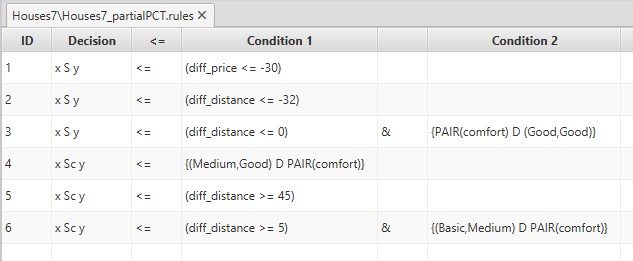
\includegraphics[width=.7\paperwidth]{raw/rules}}
	\caption{Rules tab from Houses7}
\end{figure*}

In this window all saved rules are displayed. Each rule consists of a conjunction of elementary conditions and a decision. Decision is always displayed on the left side. Each rule can have many conditions. Also, number of conditions in rules can vary for each rule. Values in columns can be sorted.\\

You can also export selected rules (rows) to CSV format. You can do this by selecting rows and choosing ''Copy selected rows'' option from context menu. Columns names will be used for CSV header.\\

If you click on the rule, rule statistic tab will be displayed below. It displays additional information about rule and rule statistics.

\subsection{Rule statistics window}\label{sub:rule-stat}

In this tab rules statistics are displayed with some additional information about rule.
Rules can be of certain or possible type. Indexes provided in statistics represents position of pair in PCT file.\\\\

Some most important statistics are:
\begin{itemize}
	\item \textbf{support} - number of pairs that supports this rule. Pair support rule if they belong to suggested relation and satisfies all elementary conditions.
	\item \textbf{strength} - support / number of pairs.
	\item \textbf{confidence} - also called certainty factor, defined as support / number of pairs of objects that satisfy all elementary conditions of rule.
	\item \textbf{coverage factor} - support / number of pairs that belong to relation suggested by rule.
\end{itemize}

\begin{figure*}[!ht] 
	\centering
	\makebox[\textwidth]{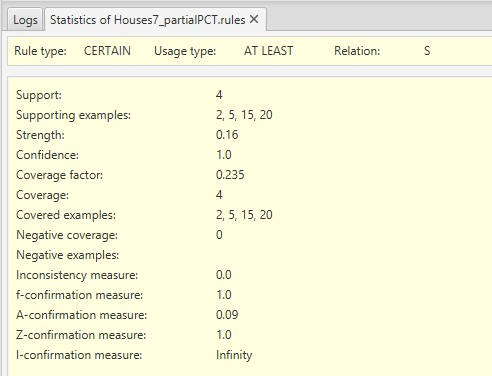
\includegraphics[width=.5\paperwidth]{raw/rules-stat}}
	\caption{Rules statistic tab from Houses7}
\end{figure*}

\vfill\newpage